\documentclass[a4paper, 12pt]{article}
\usepackage[T2A]{fontenc}
\usepackage[utf8]{inputenc}
\usepackage[english,russian]{babel}
\usepackage{amsmath, amsfonts, amssymb, amsthm, mathtools, misccorr, indentfirst, multirow}
\usepackage{wrapfig}
\usepackage{graphicx}
\usepackage{subfig}
\usepackage{adjustbox}
\usepackage{pgfplots}

\usepackage{siunitx}

\usepackage{geometry}
\geometry{top=20mm}
\geometry{bottom=20mm}
\geometry{left=20mm}
\geometry{right=20mm}
\newcommand{\angstrom}{\textup{\AA}}
\begin{document}
\begin{titlepage}
    \newpage
    \begin{center}
     Министерство науки и высшего образования Российской федерации \\ ФЕДЕРАЛЬНОЕ ГОСУДАРСТВЕННОЕ АВТОНОМНОЕ \\ ОБРАЗОВАТЕЛЬНОЕ УЧРЕЖДЕНИЕ ВЫСШЕГО ОБРАЗОВАНИЯ \\ «МОСКОВСКИЙ ФИЗИКО-ТЕХНИЧЕСКИЙ ИНСТИТУТ \\ (НАЦИОНАЛЬНЫЙ ИССЛЕДОВАТЕЛЬСКИЙ УНИВЕРСИТЕТ)» \\ (МФТИ, Физтех)
    \end{center}
    
    \vspace{15em}
    
    \begin{center}
    КАФЕДРА ТВЕРДОТЕЛЬНОЙ ЭЛЕКТРОНИКИ \\
    \vspace{1em}
    ОТЧЕТ\\
    ПО ЛАБОРАТОРНОЙ РАБОТЕ \\
    \vspace{1em}
    ФОТОЭЛЕКТРИЧЕСКИЙ СПОСОБ ПРЕОБРАЗОВАНИЯ ЭНЕРГИИ \\ СОЛНЕЧНОГО ИЗЛУЧЕНИЯ
    \end{center}

    \vspace{10em}
    \begin{flushleft}
        Работу выполнили \hspace{17em} \underline{\hspace{3cm}}
        И.Д. Бессонов \\
         \hspace{26em} \underline{\hspace{3cm}} Е.С. Иванова \\
          \hspace{26em} \underline{\hspace{2.6cm}} Е.О. Коробкина\\
        \hspace{26em}
        \raisebox{-\baselineskip}{\shortstack{\underline{\hspace{3cm}}\\(подпись, дата)}}     
        И.С. Потапова
    \end{flushleft}

    \vspace{1em}

    \begin{flushleft}
        Работу принял, оценка
        \hspace{15em}
        \raisebox{-\baselineskip}{\shortstack{\underline{\hspace{5cm}}\\(подпись, дата, оценка)}}
    \end{flushleft}

    \vspace{5em}
    
    \begin{center}
        Долгопрудный, 2025
    \end{center}
\end{titlepage}

\newpage
\tableofcontents

\newpage
\section{Аннотация}
\textbf{Цель работы:}
Исследовать темновую и световую ВАХ фотоэлемента, оценить влияние мощности падающего излучения на характеристики образца с помощью фильтров. 
    
 \section{Теоретическая часть} 
 
Прямое преобразование лучистой энергии Солнца в электрическую оcуществляется на потенциальном барьере, или так называемого вентильного фотоэффекта, суть которого - возникновение фото-ЭДС при освещении контактов металл-полупроводник и $p-n$ переходов. Однако, вследствие сложной микроструктуры контактов полупроводника с металлом, мы ограничимся в дальнейшем случаем $p-n$ перехода. 
Пусть два проводника $p-$ и $n-$ типов приводятся в хороший контакт по одной из плоскостей.
\subsection{Строение p-n перехода} 

Под действием градиента концентрации дырки из приконтактного 
слоя $p-$области будут диффундировать в $n-$область, а электроны – из $n-$области в $p-$область. 

\begin{wrapfigure}{r}{0.4\textwidth} 
    \centering
    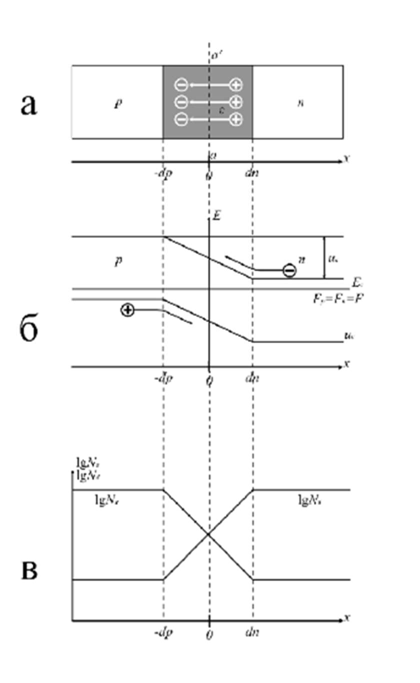
\includegraphics[width=\linewidth]{img/p-n.png} % 
    \caption{p-n переход}
\end{wrapfigure}
В результате диффузии в приконтактном слое $p-$области создается отрицательный объемный заряд нескомпенсированных ионов акцепторной примеси, а в приконтактном слое $n-$области – положительный объемный заряд нескомпенсированных ионов 
донорной примеси. Порожденное зарядами электрическое поле 
будет препятствовать дальнейшей диффузии. При этом 
напряженность электрического поля и толщины слоев объемных 
зарядов будут возрастать до тех пор, пока не достигнут своих 
равновесных знасчений, при которых диффузионные потоки 
основных носителей зарядов будут полностью скомпенсированы 
дрейфовыми потоками, вызванными электрическим полем 
объемных зарядов. Толщина такого $p-n$ перехода для различных полупроводниковых систем может изменяться от единицы и до сотых долей миллиметров, а величина напряженности электрического поля значений порядка $10^7$ В$\cdot \text{см}^{-1}$.
Состояние $p-n$ перехода в термодинамическом равновесии легко 
понять, обращаясь к его энергетической диаграмме (Рис. 1, б). 

Здесь $E_c$ – дно зоны проводимости, $E_v$ – потолок валентной зоны, $F$ – уровень Ферми. Электроны из $n-$области не могут проникнуть в $p-$область, так как для этого им необходимо преодолеть потенциальный барьер, величина которого равна контактной разности потенциалов.  



\section{Экспериментальная часть}
\begin{figure}[!h]
    \centering
    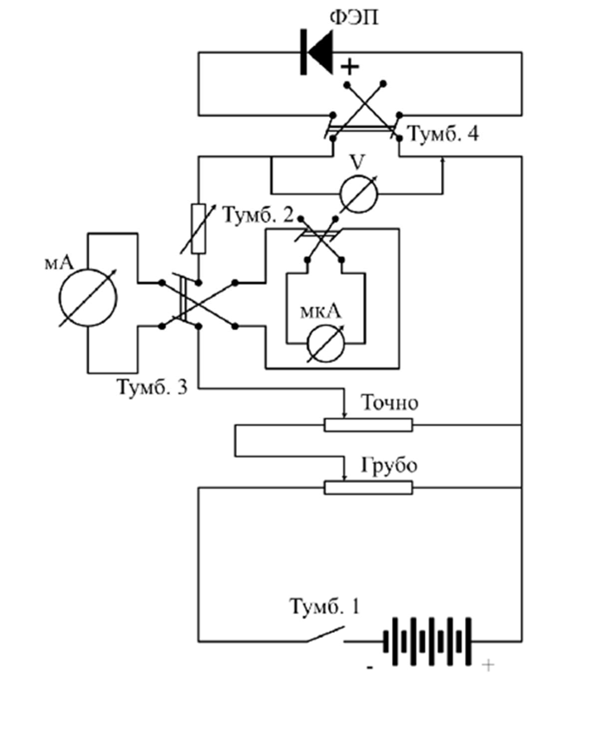
\includegraphics[width=0.5\linewidth]{img/scheme.png}
    \caption{Электрическая схема установки для экспериментальных исследований световой и темновой ВАХ фотоэлементов.}
\end{figure}

\subsection{Измерение темновой ВАХ}
Накроем фотопреобразователь сверху крышкой -- в таком режиме он может быть представлен как диод и генератор постоянного тока, включенные параллельно. Подадим на него напряжение с источника и измерим прямую и обратную ветви вольт-амперной характеристики фотопреобразователя, которые исходя из теории будут напоминать ВАХ полупроводникового диода. Результаты измерений представлены в таблицах 1 и 2, отразим их также на графике зависимости рисунок 3.

    \begin{table}[h!]
    \centering
    \begin{tabular}{|c|c|c|c|c|c|c|c|c|c|c|c|}
    \hline
        № & 1 & 2 & 3 & 4 & 5 & 6 & 7 & 8 & 9& 10 & 11 \\ \hline
        $U$, В & 0,67 & 1,34 & 2,13 & 2,85& 3,51 & 4,20 & 4,63 & 1,59 & 2,30 & 3,18 & 3,76 \\ \hline
        $I$, мкА & 3,59 & 10,52 & 27,44 & 59,86 & 124,84 & 280,24 & 482,04 & 14,76 & 33,7 & 86,96 & 168,36 \\ \hline
    \end{tabular}
    \caption{Результаты измерения прямой ветви темновой ВАХ фотопреобразователя.}
    \label{table_dark_forward_VAC}
    \end{table}

 \begin{table}[h!]
    \centering
    \begin{tabular}{|c|c|c|c|c|c|c|c|c|c|c|c|}
    \hline
        № & 1 & 2 & 3 & 4 & 5 & 6 & 7 & 8 & 9& 10 \\ \hline
        $U$, В & -0,71 & -1,30 & -1,98 & -2,59 & -3,33 & -4,05 & -4,71 & -5,30 & -6,24 & -6,85 \\ \hline
        $I$, мкА & -2,11 & -3,43 & -4,74 & -5,84 & -7,16 & -8,48 & -9,66 & -10,85 & -12,67 & -13,94 \\ \hline
    \end{tabular}
    \caption{Результаты измерения обратной ветви темновой ВАХ фотопреобразователя.}
    \label{table_dark_forward_VAC}
    \end{table}
\newpage

\begin{figure}[h!]
    \centering % Выравнивание по центру
    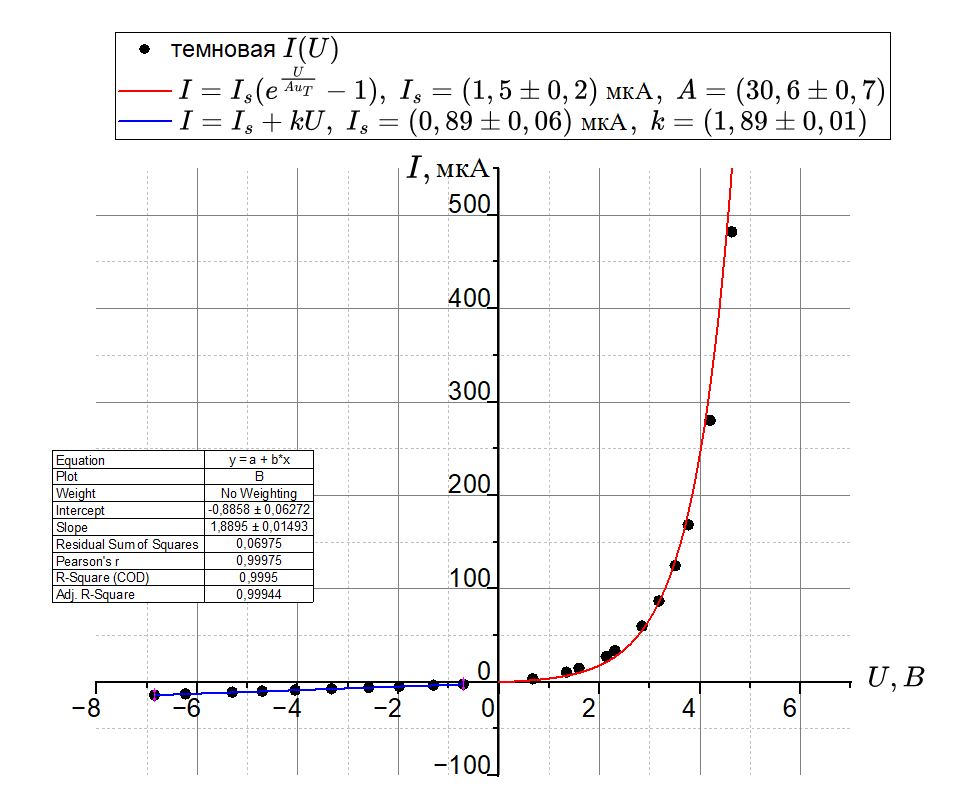
\includegraphics[width=10cm,height=8cm]{темновая.png} % Сначала вставка изображения
    \caption{Темновая ВАХ фотопреобразователя}\label{fig:sun} % Затем подпись (caption)
\end{figure}

Для прямой ветви аппроксимация задается уравнением Шокли:
$$
        I = I_s \left[ e^{ \frac{eU}{AkT}} - 1 \right] = I_s \left[ e^{\frac{U}{Au_T} } - 1 \right], 
        \label{formula_Shokli}
    $$

    где $\boxed{I_s=(1,5\pm0,2) \; \text{мкА}}$ -- ток насыщения, $\boxed{A=(30,6\pm0,7)}$ -- коэффициент неидеальности, $u_T = \frac{k_{Б}T}{e}$ = 26 мВ -- тепловой потенциал. Также из графика прямой ветви по части с большими напряжениями оценим последовательное сопротивление фотопреобразователя:
$$   
\boxed{R_{\text{посл}} = \frac{dU_{\text{прям}}}{dI_{\text{прям}}} = 828 \; \text{кОм}}.
$$

Аппроксимируем обратную ветвь графика прямой, тогда ее коэффициент наклона будет характеризовать величину шунтирующего сопротивления фотопреобразователя, а пересечение с осью ординат будет давать величину тока насыщения. Отсюда 

$$
        \boxed{I_s = (0,89 \pm 0,06)\ мкА} \quad, \quad \boxed{R_{шунт} = 1 / 1,89 = (529 \pm 3)\ кОм}.
        
$$


\subsection{Измерение световой ВАХ}
Откроем крышку, включим лампу и отключим напряжение. Теперь фотопреобразователь работает в режиме генерации. Изменяя управляющее сопротивление, возможно перемещаться по вольт-амперной характеристике. Таким образом, подбирая управляющее сопротивление, будем изменять силу тока и записывать соответствующее ей значение напряжения. Соответствующие измерения проведем с зеленым фильтром между фотопреобразователем и лампой. Результаты представлены в таблице 3, отразим их также на графике зависимости рисунок 4.


    
    \begin{table}[!ht]
    \centering
    \begin{tabular}{|c|c|c|c|c|c|c|c|c|c|c|c|c|}
    \hline
        № & 1 & 2 & 3 & 4 & 5 & 6 & 7 & 8 & 9 & 10 & 11 & 12 \\ \hline
        $U$, В & 4,14 & 3,94 & 3,19 & 3,6254 & 3,37 & 3,21 & 3,17 & 2,934 & 2,87 & 2,73 & 2,07 & 1,64 \\ \hline
        $I$, мкА & 453 & 518 & 768,8 & 649,8 & 723 & 773 & 779 & 829 & 840 & 869 & 900 & 917 \\ \hline
        
    \end{tabular}
    \caption{Результаты измерения световой ВАХ с зеленым фильтром.}
    \label{table_light_VAC_with_filter}
    \end{table}
\newpage
    
\begin{figure}[h!]
    \centering % Выравнивание по центру
    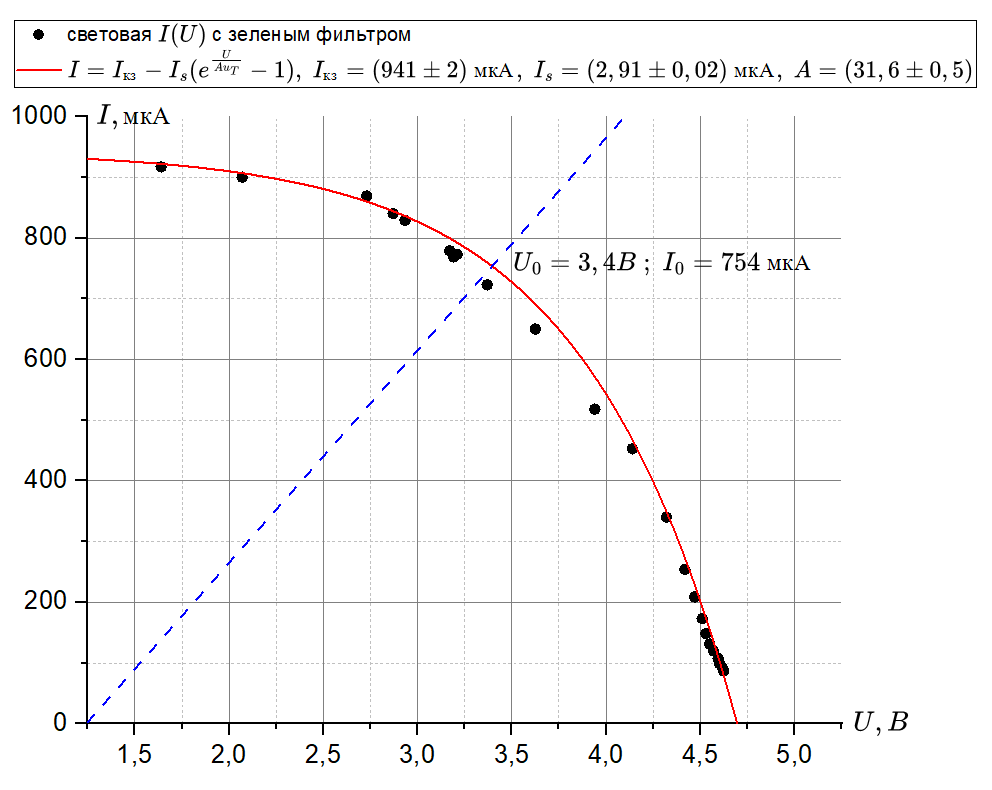
\includegraphics[width=9cm,height=8cm]{световая.png} % Сначала вставка изображения
    \caption{Световая ВАХ фотопреобразователя с зелёным фильтром}\label{fig:sun} % Затем подпись (caption)
\end{figure}

Аппроксимируем зависимость функцией Шокли, но сдвинутой по оси ординат в следствие наличия фототока неосновных носителей заряда. 

 Пересечение с осью ординат дает силу тока короткого замыкания $I_{\text{к.з.}}$: 
    \[ \boxed{I_{\text{к.з.}} = (941 \pm 2) \text{мкА}}. \]
Пересечение с осью абсцисс дает напряжение холостого хода $U_{\text{х.х.}}$:
\[\boxed{U_{\text{х.х.}} = 4.74 \text{ В}}.\]

Рассмотрим точку на вольт-амперной характеристики, задаваемую парой $(U, I)$. В этой точке достигается мощность $P = UI$, численно равная площади прямоугольника, построенному по точкам $(0,0)$ и $(U, I)$. Заметим, что мощность меняется от точки к точке и в каком-то месте ВАХ достигает максимума. Найдем максимальную мощность максимизируя площадь прямоугольника. Площадь прямоугольника:
$$
        P = UI = 941U -2,91U \left[ exp\left( \frac{U}{0,8216} \right) - 1 \right]
        \label{formula_light_VAC_equation}.
$$
Она максимальна при $\boxed{U_0 = 3,4\ \text{В}}$: $\boxed{P_{max} = 2,56\ \text{мВт}}$,при этом сила тока $\boxed{I_0 = 754\ \text{мкА}}$. Для наглядности эта точка отображена на рисунке 4.

Соответственно, для максимального КПД нагрузка должна обладать оптимальным сопротивлением 

$$
        \boxed{R_{опт} = \frac{U_0}{I_0} = 4,5\ \text{кОм}}
        \label{formula_R_opt}.
$$

Коэффициент заполнения нагрузочной характеристики 

$$
        \boxed{\xi = \frac{U_0 I_0}{U_{\text{х.х.}} I_{\text{к.з.}}} = 0,57}
        \label{formula_R_opt}.
$$

Для оценки принимая интенсивность источника с фильтром $W = 1,5\  \frac{\text{Вт}}{\text{м}^2}$(интенсивность солнечного излучения на $\lambda=550$ нм), размеры солнечной панели 15х10 см, получим КПД фотопреобразователя

  $$
        \boxed{\eta = \frac{I_0 U_0}{W S} = 11,4\%}
        \label{formula_efficiency_factor}.
 $$

\section{Выводы}
В ходе лабораторной работы изучили основные характеристики фотоэлемента, получили ВАХ без освещения и с включенным осветителем, изучили поведение тока короткого замыкания и ЭДС холостого хода при изменении освещенности. По полученным данным рассчитали основные параметры образца. 
\section{Список литературы}
\begin{itemize}
    \item\textbf{Лабораторная работа № 11а.} Фотоэлектрический способ преобразования энергии солнечного излучения., В.М. Абросимов. -- Москва: МФТИ, 2007. -- 37 с.  
\end{itemize}





\end{document}

